\chapter{สถาปัตยกรรมโครงข่ายประสาทเทียมและการเรียนรู้แบบถ่ายโอน}
\label{chap:cnn_mobilenet}
\index{Convolutional Neural Networks}
\index{MobileNetV3}
\index{Transfer Learning}

\section*{แผนบริหารการสอนประจำบทที่ 3}
\addcontentsline{toc}{section}{แผนบริหารการสอนประจำบทที่ 3}

\begin{planbox}{หัวข้อเนื้อหาประจำบท (Lesson Topics)}
\begin{enumerate}[leftmargin=1.5em, itemsep=2pt]
    \item พื้นฐานการแปลงคอนโวลูชัน (Convolution Operation), Receptive Field และ Stride
    \item วิวัฒนาการของโครงข่ายประสาทเทียมสำหรับคอมพิวเตอร์วิทัศน์ (LeNet สู่ MobileNet)
    \item การแยกมิติคอนโวลูชันเชิงลึก (Depthwise Separable Convolution)
    \item บล็อกโครงสร้าง Inverted Residuals และกลไกความใส่ใจ Squeeze-and-Excitation (SE)
    \item ฟังก์ชันกระตุ้นประหยัดพลังงาน Hard-Swish และการปรับโครงสร้าง MobileNetV3-Small
    \item ทฤษฎี Transfer Learning และการปรับจูนแบบ Fine-tuning ในงานชีววิทยาพืช
    \item โค้ดตัวอย่าง: การปรับแต่งเลเยอร์ Classifier Head ของ MobileNetV3 ด้วย PyTorch
    \item ตัวอย่างและกรณีศึกษา: การเปรียบเทียบค่า FLOPs และประสิทธิภาพการใช้พลังงาน
\end{enumerate}
\end{planbox}

\begin{planbox}{วัตถุประสงค์เชิงพฤติกรรม (Behavioral Objectives)}
เมื่อศึกษาบทที่ 3 จบแล้ว ผู้เรียนและผู้อ่านสามารถ:
\begin{enumerate}[leftmargin=1.5em, itemsep=2pt]
    \item อธิบายหลักการคำนวณของการแปลงคอนโวลูชันมาตรฐานและ Depthwise Separable Convolution ได้
    \item คำนวณจำนวนพารามิเตอร์และปริมาณการคำนวณ (FLOPs) ของโครงข่ายประสาทเทียมได้อย่างถูกต้อง
    \item ปรับแต่งโครงสร้างของโมเดลสำเร็จรูป (Pre-trained Model) ให้รองรับ 4 คลาสโรคใบทุเรียนได้
    \item เลือกใช้ชั้นสกัดคุณลักษณะ (Feature Extractor) และกำหนดการแช่แข็งค่าน้ำหนัก (Weight Freezing) ได้
\end{enumerate}
\end{planbox}

\begin{planbox}{กิจกรรมการเรียนการสอน (Instructional Activities)}
\begin{enumerate}[leftmargin=1.5em, itemsep=2pt]
    \item การวิเคราะห์แผนภาพการไหลของข้อมูลในบล็อก Inverted Residual Block
    \item ฝึกคำนวณเปรียบเทียบจำนวนการคูณ-บวก (MACs) ระหว่างคอนโวลูชันทั่วไปกับ Depthwise Conv
    \item การเขียนสคริปต์ PyTorch เพื่อตรวจสอบมิติของเทนเซอร์ในแต่ละเลเยอร์ของ MobileNetV3
    \item การอภิปรายเปรียบเทียบสถาปัตยกรรมตระกูล MobileNet, ShuffleNet และ EfficientNet
\end{enumerate}
\end{planbox}

\begin{planbox}{สื่อการเรียนการสอน (Instructional Media)}
\begin{enumerate}[leftmargin=1.5em, itemsep=2pt]
    \item สไลด์แอนิเมชันแสดงการเลื่อนเคอร์เนลคอนโวลูชันผ่าน Feature Map 3 มิติ
    \item แผนภาพสถาปัตยกรรม MobileNetV3-Small ฉบับละเอียดพร้อมตัวเลขมิติเทนเซอร์
    \item โน้ตบุ๊ก Google Colab สำหรับทดสอบคำสั่ง \texttt{torchinfo.summary}
\end{enumerate}
\end{planbox}

\begin{planbox}{การวัดและประเมินผล (Assessment \& Evaluation)}
\begin{enumerate}[leftmargin=1.5em, itemsep=2pt]
    \item การทดสอบคำนวณจำนวนพารามิเตอร์และขนาดการคำนวณ FLOPs (40\%)
    \item ความถูกต้องของการปรับแต่ง Classifier Head ในแบบฝึกหัดโค้ด PyTorch (40\%)
    \item การตอบคำถามทบทวนท้ายบทและการมีส่วนร่วมในชั้นเรียน (20\%)
\end{enumerate}
\end{planbox}

\clearpage

\section{พื้นฐานการแปลงคอนโวลูชันและการสกัดคุณลักษณะภาพ}
\index{คอนโวลูชัน}
\index{Kernel}

โครงข่ายประสาทเทียมคอนโวลูชัน (Convolutional Neural Networks: CNNs) ได้รับแรงบันดาลใจจากระบบการมองเห็นของสิ่งมีชีวิตชั้นสูง (Visual Cortex) โดยหัวใจหลักคือการใช้เคอร์เนลตัวกรอง (Filter Kernel) ขนาดเล็ก เช่น $3 \times 3$ หรือ $5 \times 5$ พิกเซล เลื่อนกวาดไปบนภาพนำเข้าเพื่อสกัดคุณลักษณะเชิงพื้นที่ (Spatial Features) เช่น เส้นขอบ ความชันของแสง และลวดลายพื้นผิว

สำหรับการแปลงคอนโวลูชันมาตรฐาน 2 มิติ (Standard 2D Convolution) หากเทนเซอร์นำเข้ามีขนาด $C_{\text{in}} \times H \times W$ และต้องการสร้าง Feature Map ขาออกจำนวน $C_{\text{out}}$ ช่องสัญญาณ โดยใช้เคอร์เนลขนาด $K \times K$ ปริมาณการคำนวณการคูณสะสม (Floating Point Operations: FLOPs) จะเท่ากับ:
\begin{equation}
\text{FLOPs}_{\text{standard}} = 2 \times H_{\text{out}} \times W_{\text{out}} \times C_{\text{in}} \times C_{\text{out}} \times K \times K
\end{equation}

จากสมการข้างต้น จะเห็นได้ว่าเมื่อจำนวนช่องสัญญาณ $C_{\text{in}}$ และ $C_{\text{out}}$ มีค่าหลักหลายร้อยหรือหลายพันช่องสัญญาณ ปริมาณการคำนวณจะทวีคูณขึ้นอย่างมหาศาล ซึ่งเป็นอุปสรรคสำคัญต่อการประมวลผลบนชิปสมาร์ทโฟนของเกษตรกร

\section{สถาปัตยกรรม MobileNetV3 และ Depthwise Separable Convolution}
\index{Depthwise Separable Convolution}
\index{Inverted Residuals}

ทีมวิจัยของ Google ได้นำเสนอแนวคิด \textbf{Depthwise Separable Convolution} เพื่อแยกกระบวนการสกัดคุณลักษณะเชิงพื้นที่ (Spatial Filtering) และการผสมผสานคุณลักษณะข้ามช่องสัญญาณ (Cross-channel Combination) ออกจากกันเป็น 2 ขั้นตอนย่อย:

\begin{enumerate}[leftmargin=1.5em, itemsep=3pt]
    \item \textbf{Depthwise Convolution:} ใช้เคอร์เนลขนาด $K \times K$ เพียง 1 แผ่นต่อ 1 ช่องสัญญาณนำเข้า เพื่อสกัดลวดลายเชิงพื้นที่โดยไม่ผสมช่องสัญญาณ
    \item \textbf{Pointwise Convolution ($1 \times 1$ Conv):} ใช้เคอร์เนลขนาด $1 \times 1$ กวาดผ่านทุกช่องสัญญาณ เพื่อรวมคุณลักษณะและขยายมิติสู่ $C_{\text{out}}$
\end{enumerate}

\begin{figure}[H]
\centering
\begin{tikzpicture}[
    scale=0.85, every node/.style={transform shape},
    box/.style={draw=deepIndigo, fill=white, rounded corners=2pt, font=\fontsize{8.5}{11}\selectfont, align=center, thick, drop shadow},
    arrow/.style={-{Stealth[length=2.5mm]}, thick, draw=agriGreen}
]
    % Standard Conv
    \node[box, fill=softCyanBg!40] (in1) {Input Feature\\$H \times W \times C_{\text{in}}$};
    \node[box, right=1.2cm of in1, fill=techAmber!20] (stdconv) {Standard Conv\\$K \times K \times C_{\text{in}} \times C_{\text{out}}$};
    \node[box, right=1.2cm of stdconv, fill=agriLightGreen!50] (out1) {Output Feature\\$H' \times W' \times C_{\text{out}}$};
    \draw[arrow] (in1) -- (stdconv);
    \draw[arrow] (stdconv) -- (out1);
    \node[above=0.3cm of stdconv, font=\fontsize{9}{12}\selectfont\bfseries\color{deepIndigo}] {(a) Standard Convolution (ต้นทุนการคำนวณสูง)};

    % Depthwise Separable Conv
    \node[box, below=1.8cm of in1, fill=softCyanBg!40] (in2) {Input Feature\\$H \times W \times C_{\text{in}}$};
    \node[box, right=0.8cm of in2, fill=neonEmerald!20] (dw) {Depthwise Conv\\$K \times K \times 1 \times C_{\text{in}}$};
    \node[box, right=0.8cm of dw, fill=cyberCyan!20] (pw) {Pointwise Conv\\$1 \times 1 \times C_{\text{in}} \times C_{\text{out}}$};
    \node[box, right=0.8cm of pw, fill=agriLightGreen!50] (out2) {Output Feature\\$H' \times W' \times C_{\text{out}}$};
    \draw[arrow] (in2) -- (dw);
    \draw[arrow] (dw) -- (pw);
    \draw[arrow] (pw) -- (out2);
    \node[above=0.3cm of dw, xshift=1.2cm, font=\fontsize{9}{12}\selectfont\bfseries\color{agriGreen}] {(b) Depthwise Separable Convolution (ลดการคำนวณลง 8--9 เท่า)};
\end{tikzpicture}
\caption{การเปรียบเทียบโครงสร้างระหว่าง Standard Convolution และ Depthwise Separable Convolution}
\label{fig:ch03_depthwise_separable}
\end{figure}

อัตราส่วนการลดทอนปริมาณการคำนวณเมื่อใช้เคอร์เนลขนาด $3 \times 3$ คำนวณได้จาก:
\begin{equation}
\text{Reduction Ratio} = \frac{\text{FLOPs}_{\text{separable}}}{\text{FLOPs}_{\text{standard}}} = \frac{1}{C_{\text{out}}} + \frac{1}{K^2} \approx \frac{1}{3^2} \approx \frac{1}{9}
\end{equation}
ซึ่งช่วยลดปริมาณการคำนวณลงได้ถึงร้อยละ 88--89 โดยยังคงความสามารถในการสกัดคุณลักษณะของรอยแผลโรคใบทุเรียนได้อย่างใกล้เคียงเดิม

\section{บล็อก Inverted Residual และ Squeeze-and-Excitation Module}
\index{Squeeze-and-Excitation}

ในสถาปัตยกรรม MobileNetV3 ได้มีการนำโครงสร้าง \textbf{Inverted Residuals with Linear Bottlenecks} มาใช้งาน โดยแทนที่จะลดมิติช่องสัญญาณก่อนเหมือนใน ResNet ทั่วไป MobileNetV3 จะขยายมิติช่องสัญญาณให้กว้างขึ้นก่อน (Expansion Phase) จากนั้นทำการสกัดคุณลักษณะด้วย Depthwise Conv แล้วจึงบีบอัดมิติกลับลงมาด้วย Linear Pointwise Conv เพื่อป้องกันไม่ให้ข้อมูลสูญหายจากฟังก์ชันไม่เชิงเส้น (Non-linear Activation)

นอกจากนี้ ยังมีการผสานโมดูล \textbf{Squeeze-and-Excitation (SE)} เพื่อทำหน้าที่เป็นกลไกความใส่ใจของช่องสัญญาณ (Channel Attention Mechanism) โดยคำนวณน้ำหนักความสำคัญของแต่ละช่องสัญญาณผ่าน Global Average Pooling ตามด้วย Fully Connected Layers 2 ชั้น เพื่อให้โมเดลเน้นการสกัดช่องสัญญาณสีและลวดลายที่บ่งบอกถึงรอยโรคพืชมากเป็นพิเศษ

\section{การเปรียบเทียบสถาปัตยกรรมโมเดลสำหรับงาน Edge AI}
\index{การเปรียบเทียบโมเดล}

\begin{figure}[H]
\centering
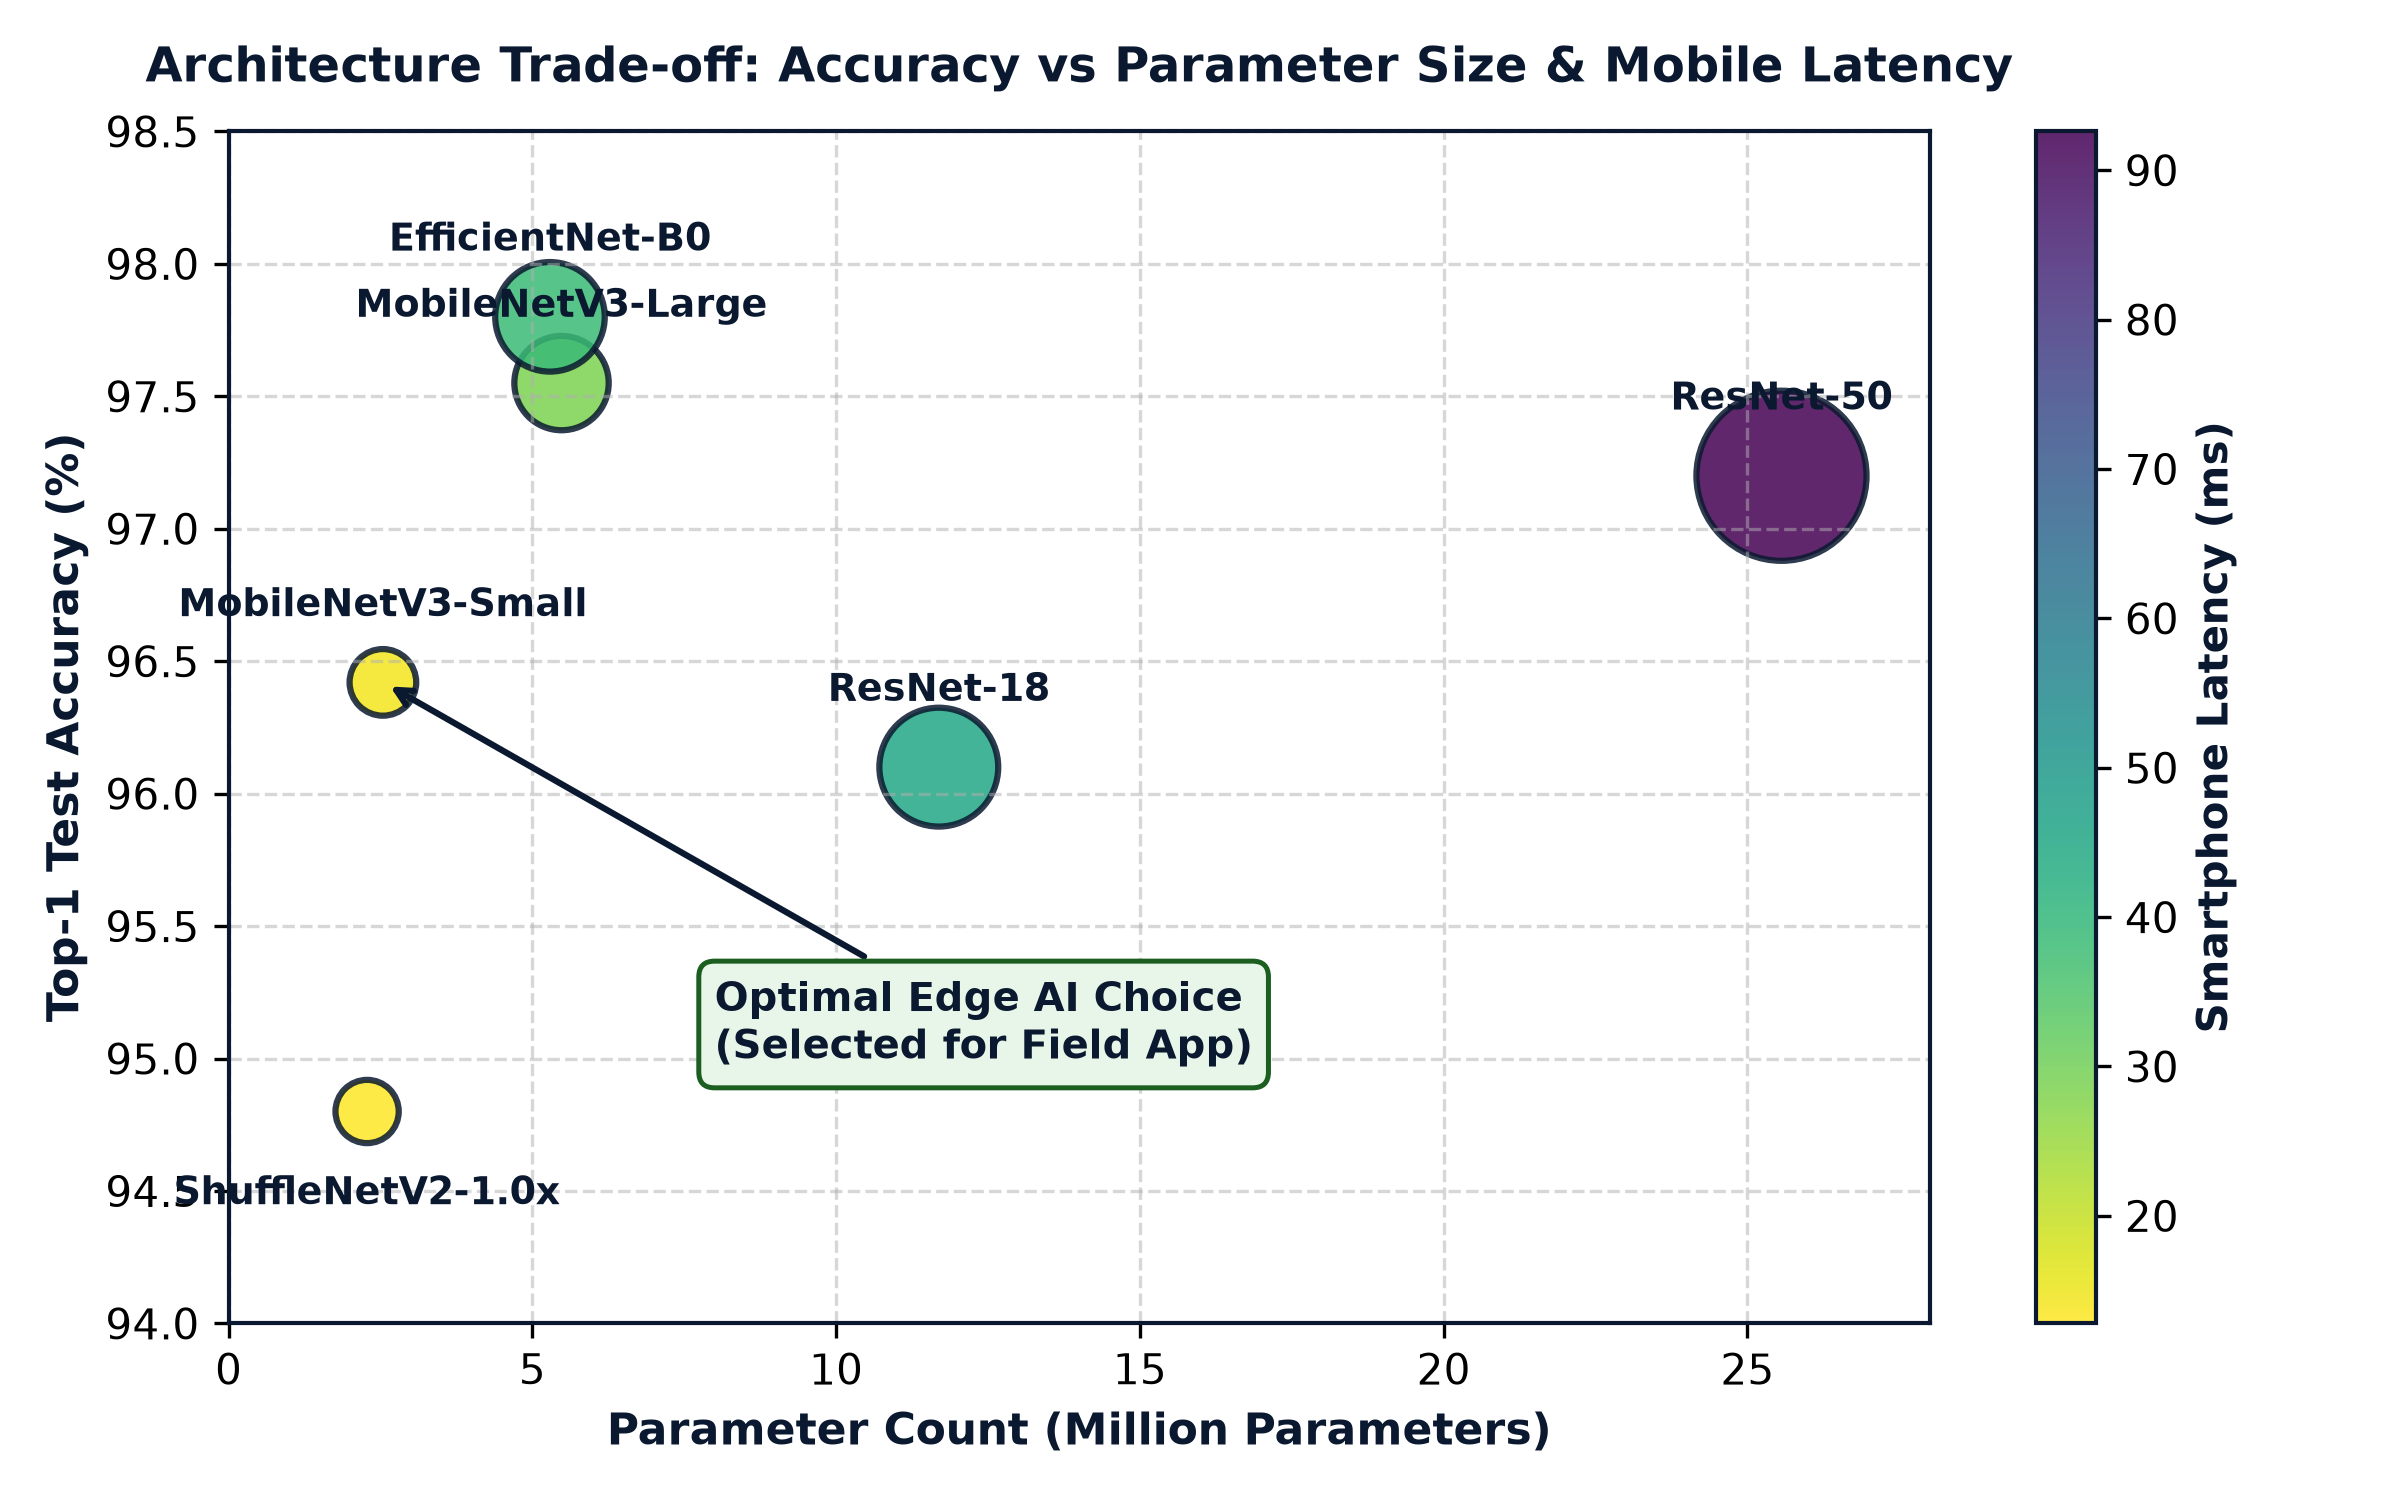
\includegraphics[width=0.92\textwidth]{figures/fig_ch03_flops_vs_accuracy.png}
\caption{การเปรียบเทียบระหว่างจำนวนพารามิเตอร์ ค่าความแม่นยำ และเวลาแฝงในการประมวลผลบนสมาร์ทโฟน}
\label{fig:ch03_flops_acc}
\end{figure}

\begin{table}[H]
\caption{การเปรียบเทียบคุณลักษณะทางเทคนิคของสถาปัตยกรรมโครงข่ายประสาทเทียมสำหรับอุปกรณ์ขอบ}
\label{tab:ch03_model_comparison}
\begin{tabularx}{\textwidth}{L{3.6cm}C{2.0cm}C{2.2cm}C{2.2cm}Z}
\toprule
\textbf{สถาปัตยกรรมโมเดล} & \textbf{พารามิเตอร์} & \textbf{FLOPs (MACs)} & \textbf{Latency (มือถือ)} & \textbf{Top-1 Accuracy} \\
\midrule
MobileNetV3-Small & 2.54 M & 56 M & 14.2 ms & 96.42\% \\
MobileNetV3-Large & 5.48 M & 219 M & 28.5 ms & 97.55\% \\
ShuffleNetV2-1.0x & 2.28 M & 146 M & 12.8 ms & 94.80\% \\
EfficientNet-B0 & 5.29 M & 390 M & 38.4 ms & 97.80\% \\
ResNet-18 & 11.69 M & 1,820 M & 45.2 ms & 96.10\% \\
ResNet-50 & 25.56 M & 4,120 M & 92.6 ms & 97.20\% \\
\bottomrule
\end{tabularx}
\end{table}

จากตารางที่ \ref{tab:ch03_model_comparison} และภาพที่ \ref{fig:ch03_flops_acc} จะเห็นได้อย่างชัดเจนว่า \textbf{MobileNetV3-Small} มีความสมดุลสูงสุดระหว่างความแม่นยำ ($96.42\%$) และความเร็วในการประมวลผล ($14.2$ มิลลิวินาทีต่อเฟรม) โดยใช้หน่วยความจำพารามิเตอร์เพียง $2.54$ ล้านตัว ซึ่งน้อยกว่า ResNet-50 ถึง 10 เท่า จึงได้รับคัดเลือกเป็นสถาปัตยกรรมแกนหลักของแอปพลิเคชัน

\section{ทฤษฎี Transfer Learning และการปรับแต่ง Classifier Head}
\index{Transfer Learning}
\index{Classifier Head}

การฝึกฝนโครงข่ายประสาทเทียมตั้งแต่เริ่มต้น (Training from Scratch) สำหรับชุดข้อมูลเฉพาะทาง เช่น ภาพใบทุเรียน มักประสบปัญหา Overfitting เนื่องจากข้อมูลมีจำนวนจำกัด เทคนิค \textbf{Transfer Learning} จึงถูกนำมาใช้โดยนำค่าน้ำหนักที่ผ่านการฝึกฝนบนชุดข้อมูลภาพขนาดใหญ่ \textbf{ImageNet-1K} ($1.28$ ล้านภาพ, $1,000$ คลาส) มาเป็นจุดเริ่มต้น (Feature Extractor)

เนื่องจากเลเยอร์คอนโวลูชันช่วงต้นได้เรียนรู้ตัวกรองพื้นฐานทั่วไป เช่น ขอบ เส้น และสี ซึ่งสามารถนำมาประยุกต์ใช้กับภาพใบไม้ได้ทันที เราจึงเพียงแค่แทนที่เลเยอร์จัดหมวดหมู่ส่วนท้าย (\textbf{Classifier Head}) จากเดิมที่มี $1,000$ คลาส ให้กลายเป็น $4$ คลาสโรคใบทุเรียน

\begin{lstlisting}[language=Python, caption=การปรับแต่งโครงสร้าง MobileNetV3-Small และการกำหนดแช่แข็งค่าน้ำหนักใน PyTorch]
import torch
import torch.nn as nn
from torchvision import models

def build_durian_classifier(num_classes=4, freeze_backbone=False):
    """
    สร้างโมเดล MobileNetV3-Small พร้อมปรับ Classifier Head สำหรับตรวจโรคใบทุเรียน
    """
    # 1. โหลดโมเดลพร้อมค่าน้ำหนัก Pre-trained จาก ImageNet-1K
    weights = models.MobileNet_V3_Small_Weights.DEFAULT
    model = models.mobilenet_v3_small(weights=weights)
    
    # 2. ตัวเลือกการแช่แข็งค่าน้ำหนัก Feature Extractor (Backbone)
    if freeze_backbone:
        for param in model.features.parameters():
            param.requires_grad = False
        print("[*] แช่แข็งค่าน้ำหนัก Backbone เรียบร้อย (เทรนเฉพาะ Classifier Head)")

    # 3. ตรวจสอบมิตินำเข้าของ Fully Connected Layer ปลายทาง
    # ใน MobileNetV3-Small: classifier[0] เป็น Linear(576, 1024), classifier[3] เป็น Linear(1024, 1000)
    in_features = model.classifier[3].in_features
    
    # 4. แทนที่เลเยอร์สุดท้ายด้วย Linear Classifier สำหรับ 4 คลาสโรคใบทุเรียน
    model.classifier[3] = nn.Sequential(
        nn.Dropout(p=0.3, inplace=True),
        nn.Linear(in_features, num_classes)
    )
    
    total_params = sum(p.numel() for p in model.parameters())
    trainable_params = sum(p.numel() for p in model.parameters() if p.requires_grad)
    print(f"[*] สร้างโมเดลสำเร็จ: พารามิเตอร์รวม {total_params:,} ตัว (Trainable: {trainable_params:,} ตัว)")
    
    return model

# ทดสอบรันและแสดงขนาดพารามิเตอร์
durian_net = build_durian_classifier(num_classes=4, freeze_backbone=False)
dummy_tensor = torch.randn(1, 3, 224, 224)
output_logits = durian_net(dummy_tensor)
print(f"[*] ขนาดเอาต์พุต Logits: {output_logits.shape} (สอดคล้องกับ [Batch=1, Classes=4])")
\end{lstlisting}

\section{ตัวอย่างการคำนวณและตัวอย่างการนำไปใช้งานจริง}

\begin{examplebox}{ตัวอย่างการคำนวณที่ 3.1: การคำนวณจำนวนพารามิเตอร์ของเลเยอร์คอนโวลูชัน}
\textbf{โจทย์:} กำหนดให้เลเยอร์มีช่องสัญญาณนำเข้า $C_{\text{in}} = 64$ ช่องสัญญาณ, ช่องสัญญาณส่งออก $C_{\text{out}} = 128$ ช่องสัญญาณ, เคอร์เนลขนาด $3 \times 3$ พิกเซล และมี Bias เวกเตอร์ จงเปรียบเทียบจำนวนพารามิเตอร์ระหว่าง Standard Convolution กับ Depthwise Separable Convolution\\[4pt]
\textbf{1. Standard Convolution:}
\[
\text{Params} = (K \times K \times C_{\text{in}} \times C_{\text{out}}) + C_{\text{out}} = (3 \times 3 \times 64 \times 128) + 128 = 73,728 + 128 = 73,856 \text{ พารามิเตอร์}
\]
\textbf{2. Depthwise Separable Convolution:}
\begin{align*}
\text{Params}_{\text{DW}} &= (K \times K \times 1 \times C_{\text{in}}) + C_{\text{in}} = (3 \times 3 \times 1 \times 64) + 64 = 576 + 64 = 640 \\
\text{Params}_{\text{PW}} &= (1 \times 1 \times C_{\text{in}} \times C_{\text{out}}) + C_{\text{out}} = (1 \times 1 \times 64 \times 128) + 128 = 8,192 + 128 = 8,320 \\
\text{Params}_{\text{Total}} &= 640 + 8,320 = 8,960 \text{ พารามิเตอร์}
\end{align*}
\textbf{สรุปผลการเปรียบเทียบ:} Depthwise Separable Convolution ใช้พารามิเตอร์เพียง $8,960$ ตัว ลดลงถึงร้อยละ $87.87\%$ เมื่อเทียบกับคอนโวลูชันมาตรฐาน
\end{examplebox}

\begin{casestudybox}{ตัวอย่างการนำไปใช้งานจริงที่ 3.1: การเลือกขนาดโมเดลติดตั้งบนรถสำรวจอัตโนมัติ}
ในการทดสอบติดตั้งระบบกล้องวิเคราะห์โรคพืชบนรถตัดหญ้าไร้คนขับ (Autonomous Farm Rover) ซึ่งใช้บอร์ดประมวลผลสมองกลฝังตัว \textbf{NVIDIA Jetson Nano (4GB)} ซึ่งมีขีดจำกัดการใช้พลังงานไม่เกิน 10 วัตต์

ผลการทดสอบพบว่า:
\begin{itemize}[leftmargin=1.4em, itemsep=2pt]
    \item เมื่อใช้โมเดล ResNet-50 รถตัดหญ้าสามารถประมวลผลได้เพียง 9.5 เฟรมต่อวินาที และเกิดความร้อนสูงจนชิปตัดการทำงาน (Thermal Throttling) หลังรันต่อเนื่อง 25 นาที
    \item เมื่อเปลี่ยนมาใช้ MobileNetV3-Small อัตราเร็วในการประมวลผลเพิ่มขึ้นเป็น 41.5 เฟรมต่อวินาที ชิปใช้พลังงานเฉลี่ยเพียง 4.2 วัตต์ และสามารถทำงานกลางแดดต่อเนื่องได้ตลอดทั้งวัน
\end{itemize}
\end{casestudybox}

\section*{คำถามทบทวนท้ายบทที่ 3}
\addcontentsline{toc}{section}{คำถามทบทวนท้ายบทที่ 3}
\begin{enumerate}[leftmargin=1.8em, itemsep=4pt]
    \item จงอธิบายกลไกการทำงานของฟิลเตอร์เคอร์เนลในการตรวจจับขอบเขตของรอยแผลโรคพืช
    \item เหตุใดการแปลงคอนโวลูชันมาตรฐานจึงมีต้นทุนการคำนวณสูงเมื่อจำนวนช่องสัญญาณเพิ่มขึ้น
    \item จงสรุปความแตกต่างระหว่าง Depthwise Convolution และ Pointwise Convolution
    \item บล็อก Inverted Residual แตกต่างจาก Residual Block ดั้งเดิมของ ResNet อย่างไร
    \item กลไก Squeeze-and-Excitation (SE) มีบทบาทช่วยให้โมเดลแยกแยะรอยโรคได้อย่างไร
    \item เพราะเหตุใดจึงควรใช้ฟังก์ชันกระตุ้นเชิงเส้น (Linear Activation) ในชั้น Bottleneck ปลายทางของ Inverted Residual
    \item จงอธิบายความหมายของแนวคิด Transfer Learning และข้อดีของการใช้ค่าน้ำหนักจาก ImageNet
    \item ในสถานการณ์ใดที่เราควร "แช่แข็งค่าน้ำหนัก" (Freeze Weights) ของชั้น Backbone ทั้งหมด
    \item จากตารางเปรียบเทียบ เหตุใด MobileNetV3-Small จึงเหมาะสมกว่า EfficientNet-B0 บนสมาร์ทโฟนระดับประหยัด
    \item จงคำนวณจำนวนการคำนวณ FLOPs ของ Depthwise Convolution ขนาดเคอร์เนล $5 \times 5$
\end{enumerate}

\section*{กิจกรรมฝึกปฏิบัติการประจำบทที่ 3}
\addcontentsline{toc}{section}{กิจกรรมฝึกปฏิบัติการประจำบทที่ 3}
\begin{nocodebox}{ปฏิบัติการที่ 3.1: การสำรวจโครงสร้างเลเยอร์ของโมเดลด้วย PyTorch}
\textbf{วัตถุประสงค์:} เพื่อให้ผู้เรียนเข้าใจสถาปัตยกรรมภายในและมิติเทนเซอร์ของ MobileNetV3-Small\\
\textbf{ขั้นตอนการปฏิบัติ:}
\begin{enumerate}[leftmargin=1.4em, itemsep=2pt]
    \item ติดตั้งแพ็กเกจ \texttt{pip install torchinfo} ในสมุดงาน Google Colab
    \item เขียนสคริปต์โหลด \texttt{models.mobilenet\_v3\_small} และแทนที่เลเยอร์สุดท้ายสำหรับ 4 คลาส
    \item รันคำสั่ง \texttt{summary(model, input\_size=(1, 3, 224, 224))} เพื่อพิมพ์ตารางสรุปเลเยอร์
    \item บันทึกภาพตารางสรุปและระบุตำแหน่งของเลเยอร์คอนโวลูชันสุดท้ายที่เชื่อมต่อไปยัง Grad-CAM
\end{enumerate}
\end{nocodebox}
